
%(BEGIN_QUESTION)
% Copyright 2007, Tony R. Kuphaldt, released under the Creative Commons Attribution License (v 1.0)
% This means you may do almost anything with this work of mine, so long as you give me proper credit

Draw the necessary connecting wires, and any additional electronic components necessary (complete with values if applicable), to make the loop-powered transmitter input a signal to channel Ain2 of the DAQ unit.  Assume an analog input range of 0 to +2.4 volts (i.e. full 20 mA signal from the transmitter should not produce a voltage at the DAQ input more than +2.4 volts, Ain2 terminal positive with respect to ground):

$$\includegraphics[width=15.5cm]{i02660x01.eps}$$

\underbar{file i02660}
%(END_QUESTION)





%(BEGIN_ANSWER)

8 points for completely correct diagram, 2 points for correct resistor value.

\vskip 10pt

One possible solution:

$$\includegraphics[width=15.5cm]{i02660x02.eps}$$

Another possible solution:

$$\includegraphics[width=15.5cm]{i02660x03.eps}$$

%(END_ANSWER)





%(BEGIN_NOTES)


{\bf This question is intended for exams only and not worksheets!}

%(END_NOTES)


